\begin{enumerate}
	\item Exercício
	
	\begin{figure}[htb]
		\caption{Integrais duplas - Aula 1 - Exercício I e II}
		\label{v01_a01_e01}
		\centering
		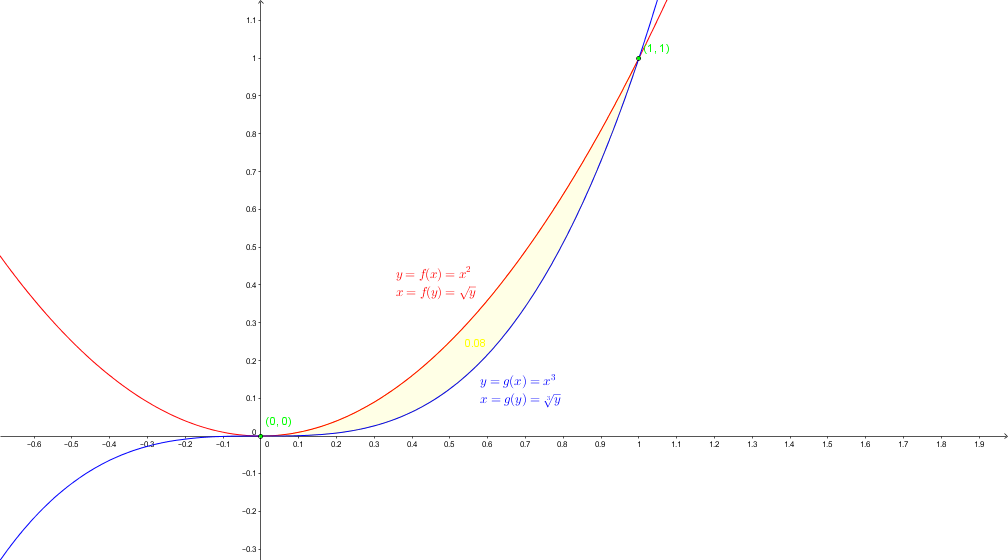
\includegraphics[width=0.5\textwidth]{v01_a01_e01.png}		
	\end{figure}
	
	\begin{equation*}
		f(x) = x^2;\; g(x) = x^3
	\end{equation*}			
	\begin{equation*}
		x = 0 \Rightarrow f(0) = g(0) \Rightarrow 0^2 = 0^3
	\end{equation*}
	\begin{equation*}
		x = 1 \Rightarrow f(1) = g(1) \Rightarrow 1^2 = 1^3
	\end{equation*}
	\begin{gather*}
		a = \int_0^1 dx \int_{g(x)}^{f(x)} dy = \int_0^1 dx \int_{x^3}^{x^2} dy = \int_0^1 dx\, [y]_{x^3}^{x^2} = \int_0^1 dx \left[x^2 - x^3\right] =\\ \int_0^1 x^2\, dx - \int_0^1 x^3\, dx = \left[\dfrac{x^3}{3} - \dfrac{x^4}{4}\right]_0^1 = \left[\dfrac{4x^3 - 3x^2}{12}\right]_0^1 = \dfrac{1}{12}\left[4x^3 - 3x^2\right]_0^1 =\\ \dfrac{1}{12}\left[x^2\left(4x - 3\right)\right]_0^1 = \dfrac{1}{12}\left[1^2\left(4 \cdot 1 - 3\right) \overstrike{- 0^2\left(4 \cdot 0 - 3\right)}\right] = \dfrac{1}{12} = 0,08\overline{3}			
	\end{gather*}
						
	\item Exercício
	
	\begin{equation*}
		f(x) = x^2 \Rightarrow f(y) = \sqrt{y};\; g(x) = x^3 \Rightarrow g(y) = \sqrt[3]{y}
	\end{equation*}
	\begin{equation*}
		y = 0 \Rightarrow f(0) = g(0) \Rightarrow \sqrt{0} = \sqrt[3]{0}
	\end{equation*}
	\begin{equation*}
		y = 1 \Rightarrow f(1) = g(1) \Rightarrow \sqrt{1} = \sqrt[3]{1}
	\end{equation*}
	\begin{gather*}
		a = \int_0^1 dy \int_{f(y)}^{g(y)} dx = \int_0^1 dy \int_{\sqrt{y}}^{\sqrt[3]{y}} dx = \int_0^1 dy\, [x]_{\sqrt{y}}^{\sqrt[3]{y}} = \int_0^1 dy \left[\sqrt[3]{y} - \sqrt{y}\right] =\\ \int_0^1 \sqrt[3]{y}\, dy - \int_0^1 \sqrt{y}\, dy = \int_0^1 y^{\frac{1}{3}}\, dy - \int_0^1 y^{\frac{1}{2}}\, dy = \left[\dfrac{y^{\frac{4}{3}}}{\left(\dfrac{4}{3}\right)} - \dfrac{y^{\frac{3}{2}}}{\left(\dfrac{3}{2}\right)}\right]_0^1 =\\ \left[\dfrac{3 \sqrt[3]{y^4}}{4} - \dfrac{2 \sqrt{y^3}}{3}\right]_0^1 = \left[\dfrac{9 \sqrt[3]{y^4} - 8 \sqrt{y^3}}{12}\right]_0^1 = \dfrac{1}{12}\left[9 \sqrt[3]{y^4} - 8 \sqrt{y^3}\right]_0^1 =\\ \dfrac{1}{12}\left[\left(9 \sqrt[3]{1^4} - 8 \sqrt{1^3}\right) \overstrike{-\left(9 \sqrt[3]{0^4} - 8 \sqrt{0^3}\right)}\right] = \dfrac{1}{12}(9 - 8) = \dfrac{1}{12} = 0,08\overline{3}
	\end{gather*}
\end{enumerate}